\documentclass{article} % For LaTeX2e
% We will use NIPS submission format
\usepackage{nips13submit_e,times}
% for hyperlinks
\usepackage{hyperref}
\usepackage{url}
% For figures
\usepackage{graphicx} 
\usepackage{subfigure} 
% math packages
\usepackage{amsmath}
\usepackage{amsfonts}
\usepackage{amsopn}
\usepackage{ifthen}
\usepackage{natbib}

\title{Project-II by Group Sydney}

\author{
Diego Antognini \& Jason Racine\\
EPFL \\
\texttt{diego.antognini@epfl.ch}, \texttt{jason.racine@epfl.ch} \\
}

\nipsfinalcopy 

\begin{document}

\maketitle

\begin{abstract}
This report provides a summary of the project two of the PCML class. The project consists of doing binary and multi-class classification on the same set of images. For both methods, we have observed that the given CNN features were more accurate than the HOG one. In binary classification, all methods were approximately equivalent except the Adaboosting and the SVM one, but we choose the SVM method as our final model because it was more stable. For the multi-class classification, neural networks and SVM were the best methods but neural networks has less variance in this case and was considered as our final model. The best way of improving our models would be to find a way to combine HOG features with the CNN one.

\end{abstract}

\section{Data Description}

The train-data for binary classification consists of $N = 6000$ images. As input we have 2 representations of the image : \textit{the histogram of oriented gradients} (HOG) $\mathbf{X}_{hog}$ and the \textit{overFEAT ImageNet CNN features} (CNN) $\mathbf{X}_{cnn}$. Our input $\mathbf{X}$ is the concatenation of $\mathbf{X}_{hog}$ with $\mathbf{X}_{cnn}$. 

Each input sample is a vector $\mathbf{x}_n$ with dimension $D = 42273$ ($5408$ for the HOG and $36865$ for the CNN) and is the concatenation of $\mathbf{x}_n^{hog}$ with $\mathbf{x}_n^{cnn}$.
The output ($\mathbf{y}$) represents the classification label of the images. For the binary classification, the label $1$  represents a car, a horse or a plane and the label $2$ anything else. For the multi-class classification, the label $1$ represents a car, $2$ a horse, $3$ a plane and $4$ anything else.

We also have test-data of size $N=11453$ without their corresponding output. Our goal is to produce predictions for those data, as well as an approximation of the test-error using \textit{Balanced Error Rate} (BER).

\subsection{Histogram of Oriented Gradients}

Histogram of oriented gradients is a feature used in computer vision in order to detect objects. To compute it, we first need to normalize the image, compute the gradients (of each pixel) for the different color channel and take those with the largest norm. Then we decompose the image in bins of size $w \times h$. For each of those bins, we compute an histogram of the orientation of the gradients using theirs angles and weighted by theirs magnitudes. The histogram has $n$ bins from $0$ to $180$ degrees. We compute this histogram using $4$ different normalizations.

In our case, the dimensions of this feature is $13 \times 13 \times 32=5408$, where the first $13$ is the number of bins in the height, the second $13$ the number of bins in the width. Finally $32$ is $4 \times 8$ where the $4$ is the different normalizations for the histogram and $8$ the number of bins (each bin has a size of $22.5°$). 

%http://lear.inrialpes.fr/people/triggs/pubs/Dalal-cvpr05.pdf
%http://vision.ucsd.edu/~pdollar/toolbox/doc/channels/hog.html
\subsection{OverFEAT ImageNet CNN features}

Those features are extracted from a convolutional network-based image features extractor OverFeat. They were trained on the ImageNet dataset (tens of millions images). The size is the output of the fifth layer of the neural network which is $1024 \times 6 \times 6 = 36864$. In our features, we also have an extra dimension which can be ruled out.

\section{Data visualization and analysis}

We first have plot the labels distribution for the binary and multi-class cases. For the binary case, we have $60.3\%$ of the data for the label $1$ and $39.8\%$ for the second one. We have observed that there is a small imbalance between the classes. For the multi-classes case, we obtain $16.07\%$, $19.37\%$, $24.87\%$ and $39.70\%$ for the labels $1$, $2$, $3$ and $4$. This time, the imbalance is more important, especially with the label $4$ and we do have to take care about it during the training.

We also wanted to analyze the distribution of our features, and have observed that for the features HOG, each of them has a similar distribution. The values are essentially in the range $[0, 0.2]$. We are also interested about the correlation between the input and output variables. We have observed that the correlation is in the range $[-0.24 ;0.30]$, and so can conclude that features seem not to have a direct correlation between them. However, a combination of features can have a high correlation with the output but we couldn't find such combination. Finally, $\mathbf{X}_{hog}$ is rank-deficient with a rank of $3467$ instead of $5408$.

For the features CNN, first we can see that it is a sparse matrix and most of the values for each data is $0$ (around $95.5\%$). This means that for each data, a small subset is able to describe the picture. Moreover, we can observe that we are faced to the problem of $D > N$ and the solution we have adopted is PCA which will describe during the next sections. The values are in mainly in the range $[0, 64.87]$. We also wanted to see the correlation of those features with the output and have found that they are in the range $[-0.24;0.18]$, which is similar to the HOG features. Finally,  $\mathbf{X}_{cnn}$ is rank-deficient with a rank of $5997$ instead of $36865$.

\section{Techniques used}

This section is a description of the techniques we have used in the project. It describes mainly how it works, why we thought it could be useful in this project and the impact of their parameters.

\begin{figure}[!ht]
\center
\subfigure[Plot of the distortion $J$ to $M$ where $M = D$ for the HOG features. The distortion decreases quickly.]{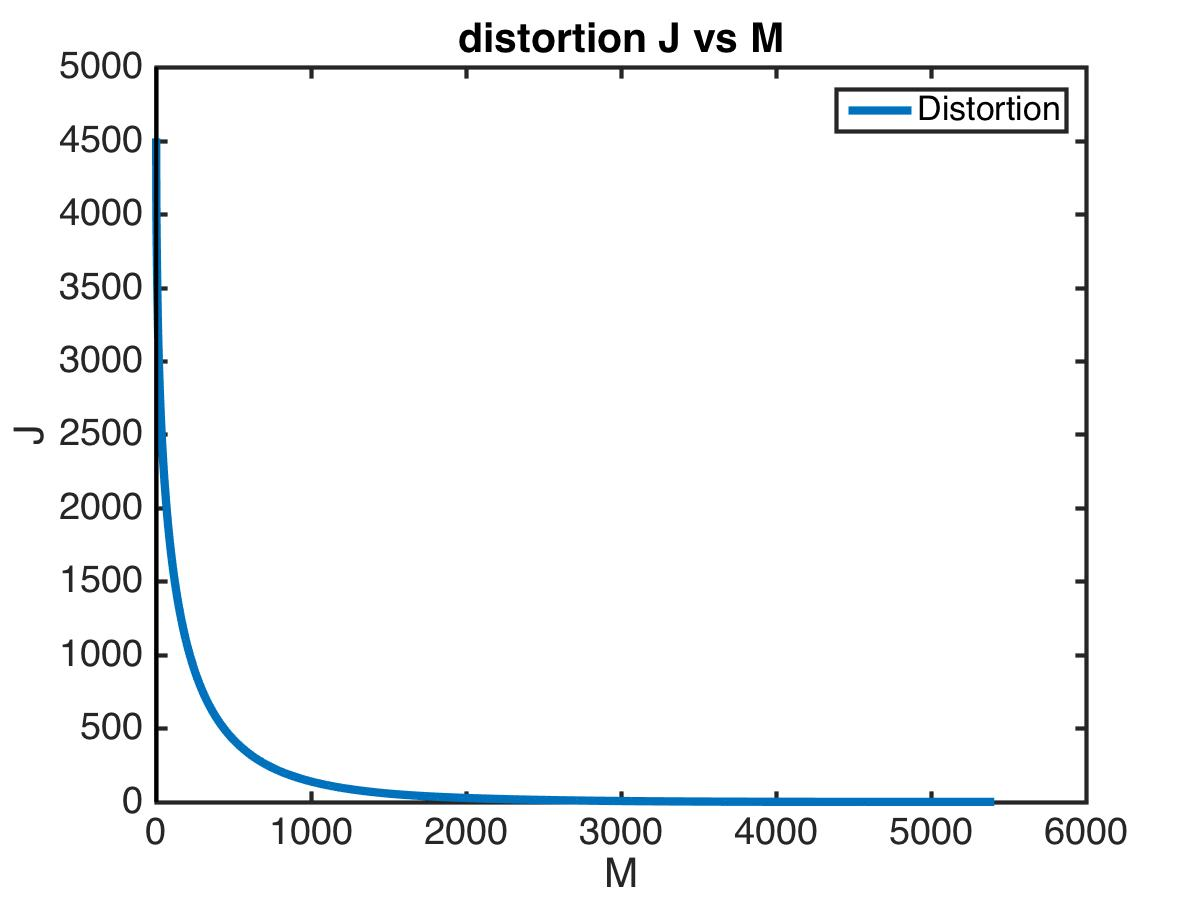
\includegraphics[width=2.7in]{figures/distortionHOG.jpg} \label{fig:distHOG}}
\hfill
\subfigure[Plot of the distortion $J$ to $M$ for the CNN features, where $M = N$ because there are too many features and so, the distortion doesn't go to $0$ and decreases slowly.]{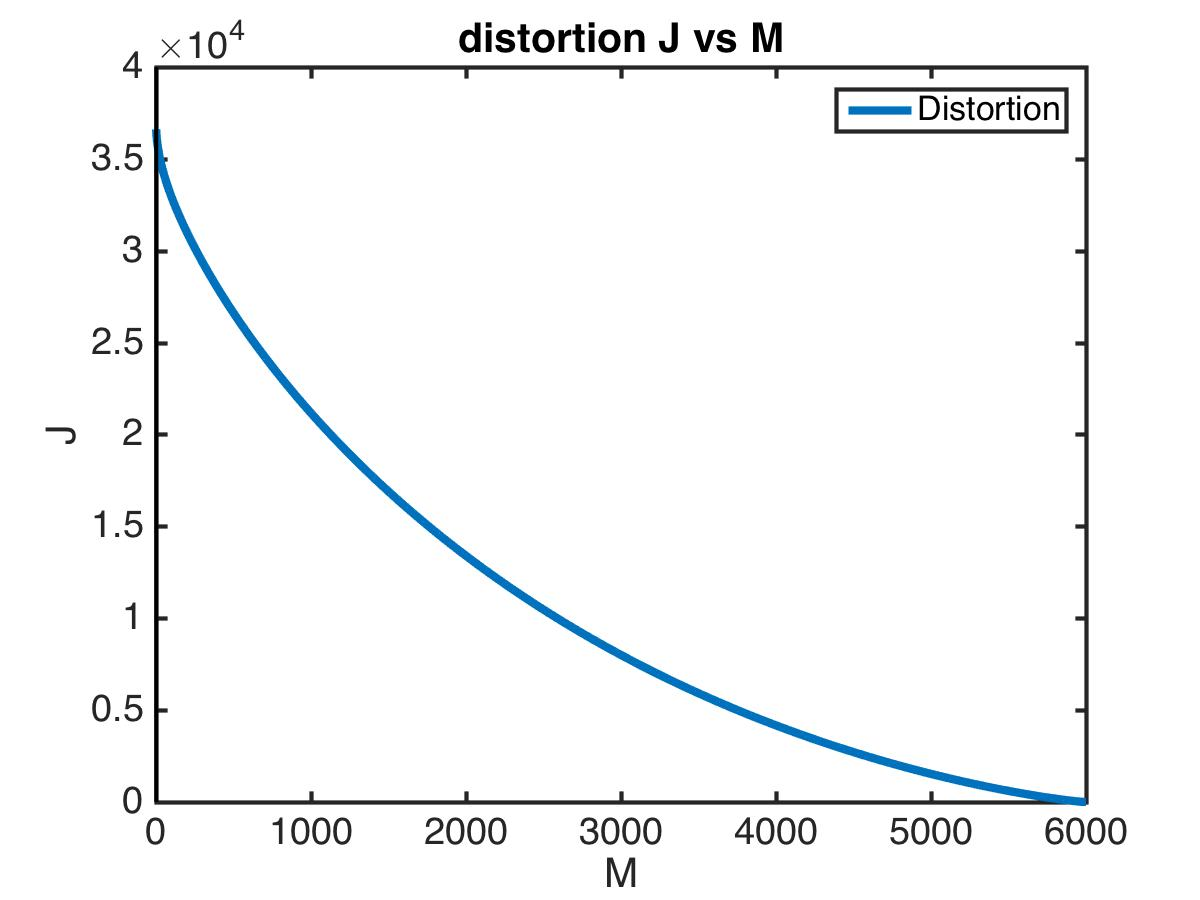
\includegraphics[width=2.7in]{figures/distortionCNN.jpg}\label{fig:distCNN}}
\hfill
\caption{}
\end{figure}

\subsection{Principal component analysis}

As we have seen in the section "Data visualization and analysis", we are faced to the $D > N$ problem mainly with the CNN features and also the HOG features depending on how we se the $k$ for the k-fold cross validation. One way to solve this problem is to use PCA.  Basically, PCA works as follow : we compute the mean and the covariance matrix $S = \frac{1}{N}\sum_{n=1}^{N}(x_n-\bar{x})(x_n-\bar{x})^T$ of our data and then compute the $M$ eigenvectors of $S$ corresponding to the $M$ largest eigenvalues. $M$ is the number of features we have to take into account in order to minimize the reconstruction. Finally, the approximation of a data sample is $\tilde{x_n} = \sum_{i=1}^M x_{ni} u_i$. However, we couldn't compute PCA using this method, because computing the full eigenvector decomposition a matrix $D \times D$ runs in  $O(D^3)$ and D is quite large. 
We have used an alternative proposed in [3] which allows us to compute the same eigenvectors in $O(N^3)$, which is roughly at least $230$ times faster. The tricks is to express $S = \frac{1}{N}XX^T$ and finally using $\frac{1}{N}XX^Tv_i = \lambda_i v_i$, where $v_i=Xu_i$, we obtain an eigenvector equation for the $N \times N$ matrix $S$.

The last parameter to set, is the parameter $M$ which defines the $M$ largest eigenvectors to take into consideration for our feature selection.We introduce a distortion measure $J = \frac{1}{N}\sum_{n=1}^{N}||x_n-\tilde{x_n}||^2$ which represents the mean squared distance between the original data sample and our approximation. Without going into the steps, the solution to the minimization of $J$ is $J = \sum_{i=M+1}^D \lambda_i$. 


The Figure \ref{fig:distHOG} shows the plot of $J$ for the HOG features. Figure \ref{fig:distCNN} shows the distortion of the CNN features, we have tried several values for $M$ and have conclude that $M_{CNN} = 150$ was a good value allowing us to compute faster results without loosing too much accuracy. The corresponding distortion might be very high compared to the HOG features, but the range of the values are not the same, CNN has values going larger than $0.2$. We tried some bigger values but we didn't get major improvements in terms of error. For the HOG features, the distortion measure seems more nice, we did the same experiments and finally set $M_{HOG}$ = $1000$. 

\subsection{Neural Networks}

This is the multi-layer perceptron (MLP) we have seen in class. The neural networks used in this project comes from the given DeepLearning matlab toolbox [1]. It uses batch sizes in order to use less memory (take the first $n$ data samples and works on them, then the next $n$ etc). We have let the default parameter ($100$). The number of epochs is simply the number of time where all the training data do a forward and a backward pass. We have put this value to $20$, in order to have a little more accuracy without loosing a lot of time, it was a good compromise because larger epochs don't mean especially better accuracy. The number of input is $M$ and output is either $2$ or $4$, depending of the type of classification (binary or multi-class). For the number of hidden layer, we have let $1$ because we didn't see improvement by adding some more. However, if this number is to high, we might overfit and so have to be careful. Having this value to $1$ might not lead to overfit. The number of neurons in the hidden layer has been tested with k-fold cross validation and we have found $1000$ for the binary classification and $700$ for the multi-class case. We also have to set up the learning rate : the optimal value we have found is $3$ for the binary case and $2$ for the multi-class one. Larger is the value, faster could be the convergence but it may diverge. By default, the activation function used is the \textit{tanh} one. We didn't see so much different using the \textit{sigmoid}. Finally, the algorithm uses stochastic gradient descent using a momentum of $0.5$, which might help to converge faster.

Neural networks are suitable for problems which might be difficult to describe in a mathematically manner and is robust to the noise, which is very useful in our case. However, we have to be careful with the weights initialization because neural networks are very sensitive to them, and especially with overfitting and computing the generalization error, this task is harder with neural networks.

\subsection{Support Vector Machine}

The normal support vector machine is a technique used for binary classification. The goal is to divide the space using an hyperplan in a way to maximize the margin, which represents the distance between closest members of the two classes. It is an interesting method because it has a regularization parameter which help to avoid overfitting. Another advantages is we can easily change the kernel function in order to try to find better boundaries. However, what is difficult is to find good parameters ($C$, $\gamma$). $\gamma$ is the kernel scale parameter which is related to how the data are scattered. We might have many support vectors and overfit if we set the $C$ too large and on the contrary if it is small, we might have not enough support vector and underfit. However, the best results we can obtain with support vector machine need to have a small imbalanced between the positive and negative examples. As seen in the section "Data visualization and analysis", there classes are not very well balanced as much for the binary classification as the multi-class classification. We have use the same algorithm we have seen in the lab $SMO$. 

We have used the method \textit{fitcecoc} in matlab. We have used k-fold cross valiation to find $C$ and $\gamma$ and have set the margin $C=1$, and $\gamma = 1$. Only the linear kernel function was available in this mode, and so, gaussian kernel might give better results. Even if the method is linear, SVM only classify directly the dataset in two classes, and so it is not a problem with the multi-class case because we always classify data in one of the two classes for the current classifier (see \textit{OVA} below).

To adapt support vector machine to a multi-class classifier, we have used \textit{One Versus All} method, which divides the problem in $4$ binary classifications. We train the data with all the classifiers and at the end, each classifier says if the data is positive to its class. If there are more than one classifier with the data sample considered as positive, we use the highest confidence to associate the class. Another possible method would have been to use \textit{One Versus One} which needs $6$ classifiers in our case, and is less sensitive to the imbalance but needs more computational resource, but it didn't give better results. 

\subsection{Bootstrap Aggregation (Bagging)}

As we have seen in the lecture, decision trees are good because the training and the prediction is quite fast, even with many features or large dataset but have a high variance and might overfit. The idea of decision trees, is to have a several questions where to answer yes/no and to move in the tree. At the end, the leaves give the corresponding class. To construct this list of questions, we divide recursively the space in a way to minimize the cost of impurity (depending of the threshold to find and the current feature). The depth of the tree is a parameter.

The idea of bootstrap aggregation is to average several decision trees. It will help to reduce the variance and avoid overfitting. It generates $m$ new training sets of the same size, by sampling uniformly and with replacement the original training set. Then we have $m$ decision trees which will grows independently with their own generated training sets. Finally, to predict the class it takes the average over all the trees. In order to find those parameters $m$ and the maximum depth of the tree, we have also used k-fold cross validation and the best values are $m = 200$ and maximum depth of $512$ for the binary classification and for the multi-class case $m = 500$ and maximum depth also of $512$. Having a high maximum depth might lead to overfit because we specialize to much the features split, but if it is too small, it might underfit because the features are not well split in order to identify classes. For the parameter $m$, it is better to have a higher number in order to have a large number of trees which can give a better accuracy of the prediction and reduce the variance.

We have used two different methods in matlab, one using \textit{fitensemble} with the parameter 'Bag' and another one which is the \textit{TreeBagger}.

\subsection{Random Forests}

The idea of random forests is similar than with bagging in a sense that we train several trees and take the average predictions. Like bagging, each trees have trained on a subset of the dataset. However, there is another aspect in random forest that bagging doesn't have: for each split, instead of searching a split among the overall features, we search only among a random subset of features. The size of this subset is a parameter $m$ as well as the maximum depth tree and the number of trees, like in bagging. Like bagging, random forests are useful because they help reducing the variance and might avoid overfitting. But the more interesting ideas is to select only a subset of the features in the split process. Moreover, it is efficient against imbalanced dataset.

As in bagging trees, the number of trees and the maximum depth tree behaves in the same manner. The last parameter $m$ has an important impact because it is too small, the subset of features might not describe correctly the data, and if it is too high, this subset might be to high and might not represent well the data. We have to find a good compromise in order to have a certain number of features to describe the data. Still with k fold cross validation, we have found for the multi-class case a maximum depth of $1024$,  $64$ trees and a $m = 20$. For $m$, an heuristic could be the square root of the number of features, but it was less efficient than $20$ in our case. For the binary case, those parameters are $1024$, $256$ and $50$.

The given Piotr matlab toolboox [2] contains a method \textit{forestTrain} which takes the defined parameters and \textit{forestApply} for the prediction.

\subsection{Adaboosting}

Adaboosting [4] is another way to average trees. If we observe more deeply the bagging approach, some trees might have a very high variance and some a very slow. Averaging all those trees decrease the variance and have a small bias. Boosting is the opposite : decrease the bias when averaging and have a small variance. In order to achieve this, each data sample has an assigned non-negative weight. After each iteration, if the data sample is misclassified, its weight is increased for the next iteration. So misclassified data samples will have more importance. The parameters are the same as in the bagging and behave in the same manner. The Piotr matlab toolboox [2] contains a method \textit{adaBoostTrain} and \textit{adaBoostApply} for the prediction. We have only used it for the binary classification, because the implementation is not adapted for more classes. However, we should have used the same technique as SVM : OVA. The parameters we obtain with k fold cross validation are $1024$ for the number of trees and $4$ for the maximum depth.

\section{Evaluation methods}

In order to evaluate our different models, we have split our data in two sets of $80\%$ and $20\%$ for the training and the test sets. We choose this percentage in order to have still enough data for the training set and also enough to estimate correctly our models on the testing set. We learn only on the training set and then use the test set in order to estimate the error using the \textit{Balanced Error Rate}. This error compute the average percentage of misclassification per class. It allows us to avoid the case of the $90\%/10\%$, predict only the class of the $90\%$ and have a good error. We have also used k-fold cross validation to tune the parameters up of our different models. We set $k=10$ because we have a lot of data, splitting them into $10$ folds seems reasonable ($4320$ data samples for the training set and $480$ for the testing set). We repeated the experiment $30$ times with different seeds in order to split the data in a unique random way for each trial and so try to have an unbiased estimation error. 

\section{Model comparison}

This section describes our models for the binary classification as well as the multi-class classification. We have essentially put our effort on the CNN features. The reason is because with only the HOG features, we couldn't get an error lower than $20\%$ for binary and multi-class classification. We have tried to take the whole matrix, only a subset of features with $M = 1000$, different methods but nothing worked. With the CNN features, we didn't have this problem. We think that the reason is because those features are too noisy : they came directly form the images. Some of them are rotated, inverted and so, the gradient is also transformed, which might be confusing for the learning. The CNN features are already computed from a convolutional neural networks which gives the features it has seen on the image with a specific weight. Because each sample has approximately $5\%$ of the overall features, they are fewer and are more specific than the HOG features.

\subsection{Binary classification}

\begin{figure}
\center
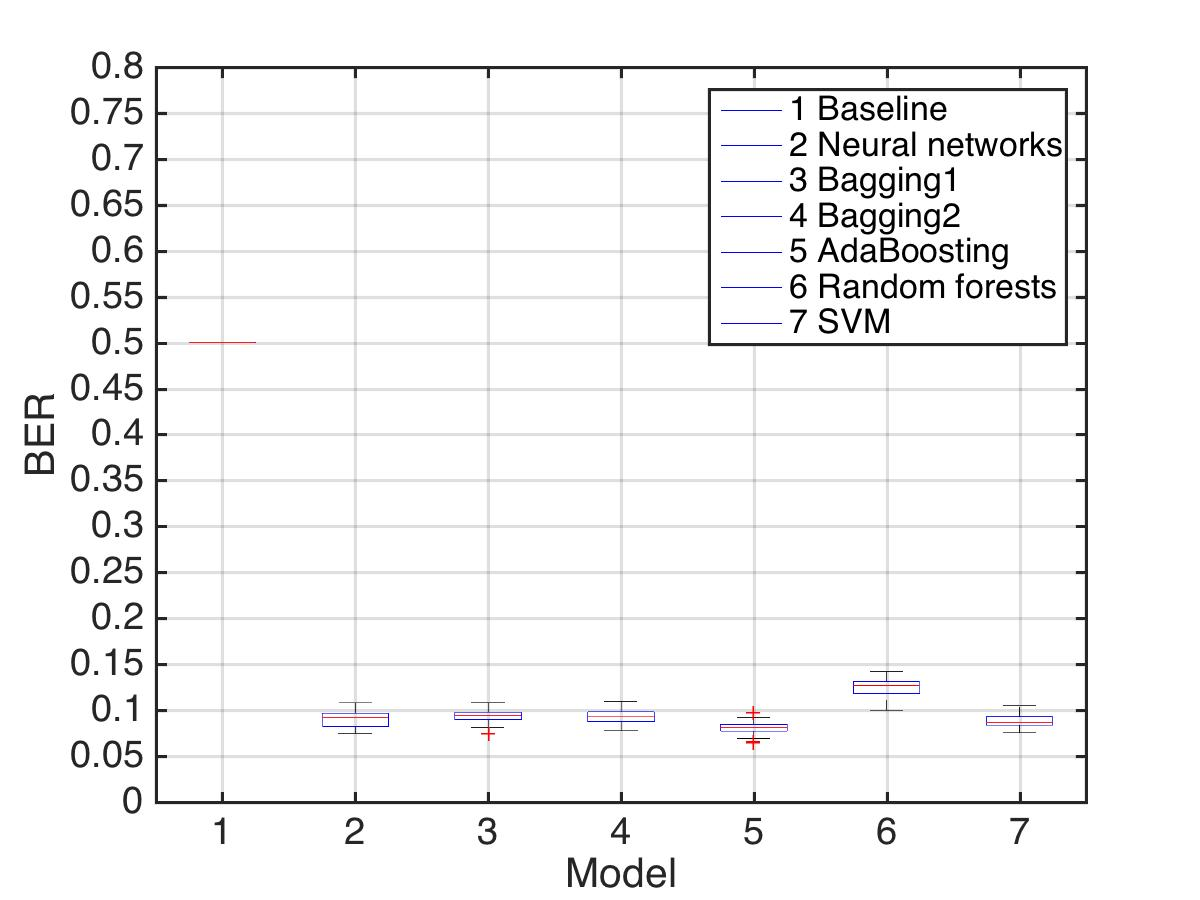
\includegraphics[width=5in]{figures/binaryclassifications.jpg} 
\caption{Boxplot of our models for the binary classification, using the BER. Each model is represented with a box where we can see their mean and their standard deviation.}
\label{fig:bin_models}
\end{figure}

The Figure \ref{fig:bin_models} represents the BER error for each models. The first model used simply returns the label $1$ to all inputs, which will allow us to compare improvements with other models. It gives us an error of $0.5$, which is obvious because all the input are in the same class and the other has none of them. The second model uses neural networks with normalized data because we got better results and because it can avoid being stuck in a local minima and might speed the training. It clearly outperforms the baseline. We can see that it has a bit of variance but has a low bias. Increasing the number of hidden layer might accentuate the variance and diminish the bias. For all other models, we didn't get improvements using normalization.

Our third and fourth model uses bootstrap aggregation with different implementations. They have similar performance than neural networks. In the first one, we can see that the variance is lower but there are some outliers. The other one has a bigger variance but is more robust to outliers. Let's remind than bagging averages trees and some trees might have big and small variance, which reduce variance in average. In general, it reduces the variance and increase slightly the bias. Compared to the neural network, the variance is better but the bias surely is worst.

The next model ($5$) is the boosting method. As in bagger, it reduces the variance because it takes the average and the bias should be lower, which is the contrary compared to the bagger. We can also see that there are some outliers, but they are still better than the other seen methods. We think that the main reason is the variance and seems to be higher than the other models. In general, boosting should be better than bagger.

Random forests is used for the sixth model. Surprisingly, we obtain worse results than the other methods. The k fold cross validation gave us better results when we were looking for the parameters. A possible cause of this effect is that it has overfit during the tuning process and so, gives worse performance in the real case. The parameter concerned should be the maximum depth which should be too high for our data because it specializes too much the features during the split. In theory, it should have better performance than the bagging and have less variances because we split only on a subset of features, however, the bias should be higher. Beside this, maybe the bias is too high and in this case, increasing the subset of feature might help to fix this.

Our last model used the SVM as the one used for the multi-class classification. It works because the SVM OVA can be adapted easily to take into account only 1 binary classifier ($\frac{2*(2-1)}{2}=1$). Compared to the other methods, we can observe that it is quite stable and have a low variance. If the parameter $C$ is set optimally, we should have a good variance and a good bias. However, if it is too high, the variance should be small but the bias could be high. In the other side, if $C$ is small, the bias should be lower but we have fewer support vectors which leads to a higher variance. However, let's remind that we use the same as in the multi-class classifier, using a linear kernel due to the implementation of matlab. If we could have changed the kernel into a non-linear one, the decision boundary would be different and might surely reduce the error. However, we would be faced to $\gamma$ which might change the variance and the bias.

Our final model will be the SVM one, because we considered it has one of the smallest error, but it doesn't have any outliers and is more stable than the Adaboosting.

We wanted to test some others models but we didn't get time to do it. First, we wanted to see if using a multi-class classifier which have a smallest error and then transform the prediction into a binary case would increase the accuracy.  We think that the error might be improved but in general, it should stay more or less the same. Another promising method we wanted to try is the \textit{fernst} one. It should outperforms other decision-based trees because they compute posteriors multiplicatively [REF]. We obtain good results with the Adaboosting method and think that fernst should produce better results.

\subsection{Multi-class classification}

\begin{figure}
\center
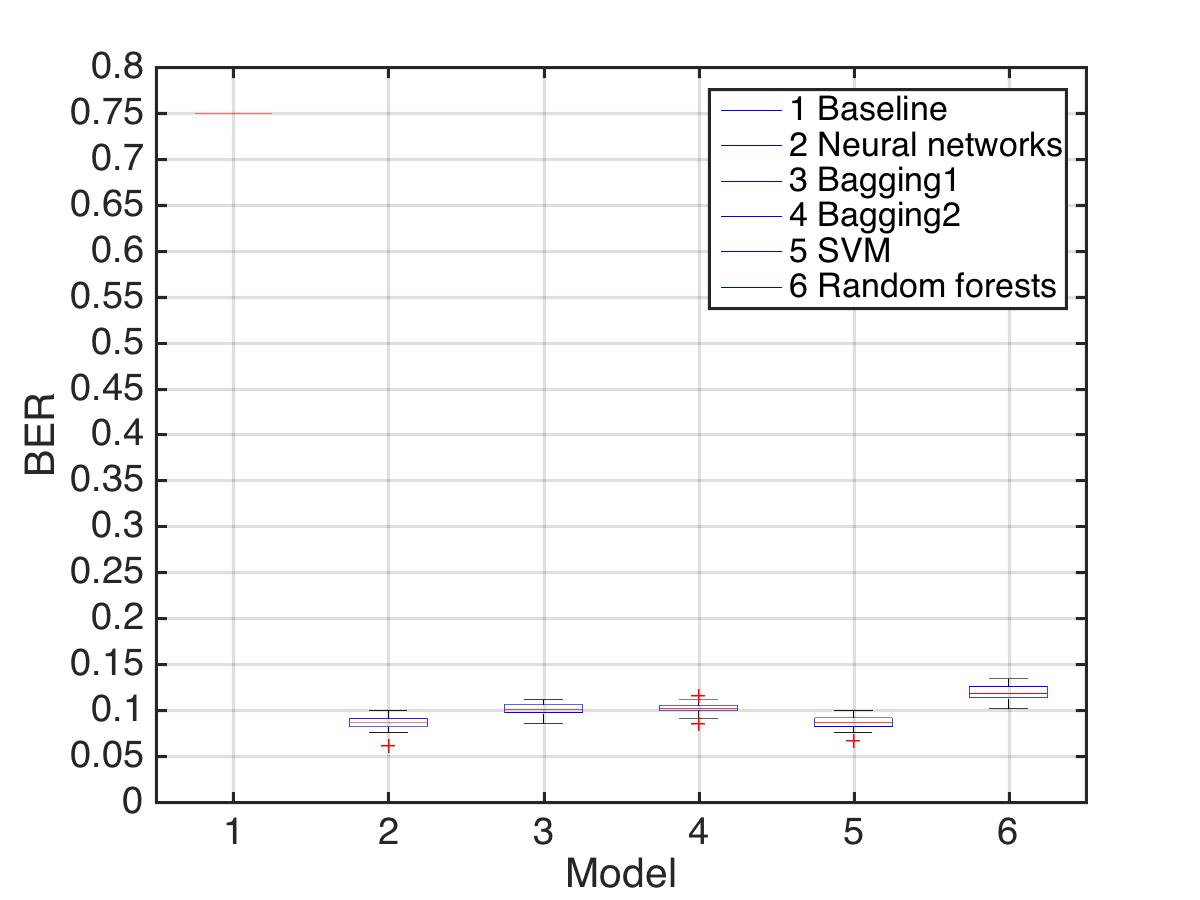
\includegraphics[width=5in]{figures/multiclassifications.jpg} 
\caption{Boxplot of our models for the multi-class classification, using the BER. Each model is represented with a box where we can see their mean and their standard deviation.}
\label{fig:mul_models}
\end{figure}

The Figure \ref{fig:mul_models} represents the BER error for each models. A general observation we can see is that the error of the models are similarly to the binary classification, which might mean that they both misclassify a shared subset of misclassified data samples. 
Another observation we might see is that in general, the variance is lower in the multi-class models. We think that the reason is that we classify explicit objects (car, horse, plane and others) without mixing them, which might be less noisy.

The first model used simply returns the label $1$ to all inputs, which will allow us to compare improvements with other models. It gives us an error of $0.75$, which is obvious because all the input are in the same class and the others has none of them. The second model uses neural networks with normalized data as explained in the binary section. We can see that even if we have more label, neural networks are still efficient and has a low bias and a little bit of variance, because there is one outlier. Obviously, neural network are a lot more efficient than our baseline.

Our third and fourth model uses bootstrap aggregation with different implementations. They are less good than neural networks. We think that the reason is because we have more labels, the set of splits to decide in which class is a data sample is more precised and so, a little bit less accurate. In the first one, we see that the variance is lower and there is no outlier comparing to the other bagger model. Those results compared to the binary classification are inverted, we might think that the implementation of those methods in matlab could be more efficient for a binary classification or multi-class classification depending of the method.

The next model ($5$) is the SVM one using the OVA method. As we said earlier, it is several binary classifiers combined together. We obtain similar results than in the binary classification because the nature of the problem is very similar : the only difference is the number of labels. Moreover, it seems to have lower variance, even if there is one outlier. As highlighted before, changing the kernel function might lead to decrease the error and could be worthwhile to implement this version, however we didn't have time to do it.

The last model uses random forests. As before, we obtain worse results than the other methods. It has greater bias than the other.
We also think that the method has overfit when using k fold cross validation in order to find optimal parameters. The parameters to be changed could be the maximum depth tree because if it is too high, the split will be very specialized. We also think that the bias could be high and so, increasing the parameter $m$ could be worthwhile because first, we may need more features to classify a data sample in one of the four classes. Secondly, because the bias is surely higher than other method as well as the variance. More training samples should help to decrease the variance and to tune the parameters up.

Our final model is neural networks and not SVM. Their error is nearly the same, however, the variance of the neural networks is much lower than the one of SVM. Even if both have one outlier and surely have the same stability. 

Beside trying \textit{fernst} method as proposed in the binary case, we wanted to try to use several multi-class classifiers and then combine their results to see which data samples were more difficult and find a way to class them with more accuracy. One of the method we wanted to use was simply voting system in a similar manner as SVM OVA. We think that it could help to decrease the error.

\section{Conclusion}

We have seen that advanced machine learning methods are efficient to solve image classification problems. The errors obtained with binary classification and multi-class classification are closed and prove that the nature of the problem is similar. We have tried different methods and have remarked that SVM model was better than the other in general. In both case, it produces good results and has a small variance. We really think that there is a way of improving it by changing the kernel function because data are surely not separate linearly. At the end, we think that the best way of improving our binary and multi-class classifier would be to find a way to combine the HOG features with the CNN ones. 

\section{References}

[1]    IMM2012-06284, R. B. Palm, "Prediction as a candidate for learning deep hierarchical models of data", 2012.


[2]    Piotr Doll\'ar, {P}iotr's {C}omputer {V}ision {M}atlab {T}oolbox ({PMT}), \url{http://vision.ucsd.edu/~pdollar/toolbox/doc/index.html}. 


[3]    Pattern Recognition and Machine Learning, Christopher Bishop, p 569-570, 2007.


[4]    R. Appel, T. Fuchs, P. Dollár, P. Perona; "Quickly Boosting Decision Trees – Pruning Underachieving Features Early," ICML 2013.
\end{document}